\documentclass[../SWD_disp.tex]{subfiles}

\begin{document}
\section{GUI Design Patterns}
Hvorfor bruge et GUI pattern?

Det kan skabe bedre workflow i teams, nemmere at teste specielt nemmer for andre at dykke ned i, hvis det skal vedligeholdes.


\subsection{MVVM}
I forhold til MVC og MVP så er MVVM mere segregreret. Her prøves der nemlig skelne helt væk fra modellen.

\begin{figure}[H]
	\centering
	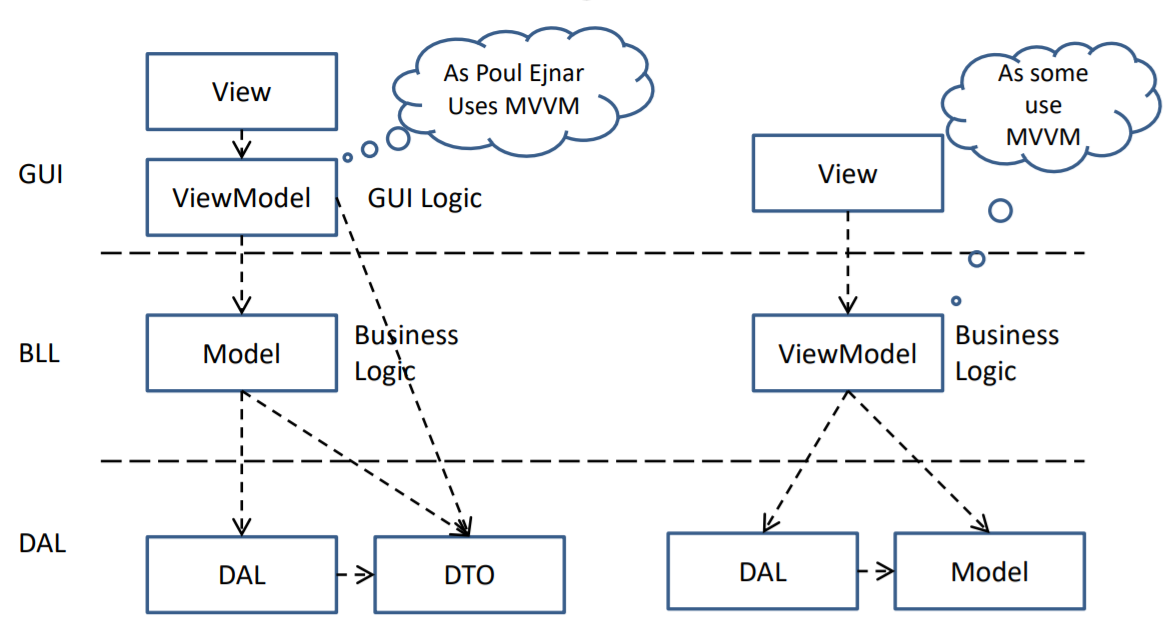
\includegraphics[width = 0.6\textwidth]{mvvm.png}
\end{figure}
\subsection{Elementer af MVVM}
\begin{enumerate}
	\item Model 
	\begin{itemize}
	\item an object model that represents the real
state content (an object-oriented
approach)
\item  the data access layer that represents that
content (a data-centric approach)
	\end{itemize}
	\item View 
	\begin{itemize}
		\item As in the classic MVC pattern, the view
refers to all elements displayed by the GUI
such as windows, buttons, graphics, and
other controls
\item A View may represent the whole window -
or it may only represent a part of a window
- typical a user control or DataTemplate
	\end{itemize}
	\item ViewModel
	\begin{itemize}
	\item The ViewModel is a “Model of the View”
\item  Meaning it is an abstraction of the View that also
serves in data binding between the View and the
Model
\item  It could be seen as a specialized aspect of what
would be a Presenter (in the MVP pattern) that
acts as a data binder/converter that changes
Model information into View information and
passes commands from the View into the Model
\item  The ViewModel exposes public:\\
– properties,\\
– commands
	\end{itemize}
\end{enumerate}


\subsection{MVC + MVP}
Brugeren interagere med ``controlleren'' som ændre på modellen, som opdatere viewet. Set på billedet under.
\begin{figure}[H]
	\centering
	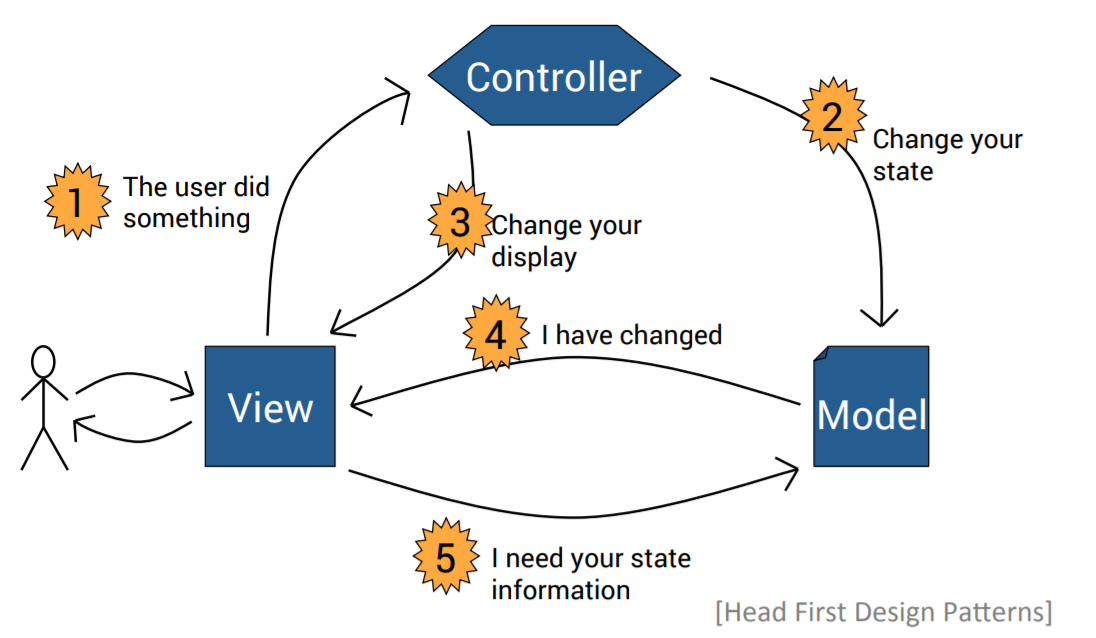
\includegraphics[width = 0.6\textwidth]{mvc.png}
\end{figure}


\subsubsection*{View}
Gives you a presentation of the model. The view usually gets the state and data it needs to display directly from the model.  
\subsubsection*{Model}
Holds all the data, state and application logic. The model is unaware of the view and controller, although it provides an interface to manipulate and retrieve its state and it can send notifications of state changes to observers 
\subsubsection*{Controller}
Takes user input and figures out what it means to the model 
\begin{itemize}
\item Make a strong separation between presentation (view \& controller) and domain (model)
\item Divide GUI widgets into a controller (for reacting to user stimulus) and view (for displaying the state of the model). Controller and view should (mostly) not communicate directly but through the model
\item Have views (and controllers) observe the model to allow multiple widgets to update without needed to communicate directly - Observer Synchronization
\item Advantage: a strong separation of model and UI, makes the application easier to update and maintain. 
\item Disadvantage: requires more code than Forms \& Controls 
\end{itemize}
\begin{enumerate}
	\item Superviser Controller
	\begin{itemize}
		\item Short description:
	Factor the UI into a view and controller where the view handles simple mapping to the
	underlying model and the controller handles input response and complex view logic
	\item Many UI frameworks provide the ability to easily map between the view and
	model, often using some kind of Data Binding
	– These approaches are very effective in allowing you to declaratively set up a
	relationship between elements in the view and model
	\item Usually, however, there are more complex relationships which require you to have
	more complex view logic
	– This logic can be hard to manage, and in particular hard to test, while embedded in the
	view
	\item Supervising Controller uses a controller both to handle input response but also to
	manipulate the view to handle more complex view logic
	– It leaves simple view behavior to the declarative system, intervening only when effects
	are needed that are beyond what can be achieved declaratively
	\item The essence of a good Supervising Controller is to do as little as possible
	– Let the view handle as much as possible and only step in when there's more complex
	logic involved 
	\end{itemize}
	\item Passive Controller
	\begin{itemize}
		 \item The View has no direct association to the
Model.
\item The View only contains the widgets that
shows the data on the screen, and it will
hand over all user input to the Presenter
(Fowler call it “Controller”)
\item The Presenter contains all the GUI logic and
is responsible for both updating the Model
and updating the View
– the Presenter populates the Widgets in the View
with data from the Model. 
	\end{itemize}
\end{enumerate}


\end{document}
